\documentclass{article}
\usepackage[utf8]{inputenc}
\usepackage{amsmath}
\usepackage{graphicx}
\usepackage{listings}
\usepackage{xcolor}
\usepackage{geometry}
\geometry{margin=1in}

\definecolor{codegreen}{rgb}{0,0.6,0}
\definecolor{codegray}{rgb}{0.5,0.5,0.5}
\definecolor{codepurple}{rgb}{0.58,0,0.82}
\definecolor{backcolour}{rgb}{0.95,0.95,0.92}

\lstdefinestyle{mystyle}{
    backgroundcolor=\color{backcolour},
    commentstyle=\color{codegreen},
    keywordstyle=\color{magenta},
    numberstyle=\tiny\color{codegray},
    stringstyle=\color{codepurple},
    basicstyle=\ttfamily\footnotesize,
    breakatwhitespace=false,
    breaklines=true,
    captionpos=b,
    keepspaces=true,
    numbers=left,
    numbersep=5pt,
    showspaces=false,
    showstringspaces=false,
    showtabs=false,
    tabsize=2
}
\lstset{style=mystyle}

\begin{document}

\title{Mini Project 4}
\author{EECE 7398 Legged Robotics}
\date{}
\maketitle

\section*{Code Listing}

\subsection*{\texttt{func\_feedback.m}}
\begin{lstlisting}[language=Matlab]
% Compute control action using feedback linearization
%
% Inputs:
%       x: states
%           q1
%           q2
%           q3
%           dq1
%           dq2
%           dq3
%       alpha: Bezier coefficients for q2 and q3
%           alpha2 (1st to 5th coefficients)
%           alpha3 (1st to 5th coefficients)
%       s_params: for gait timing
%           q1_min
%           delq
%
% Outputs:
%       u: control action
%
function u = func_feedback(x,alpha,s_params)
% gains
kp1 = 2500;
kp2 = 2500;
kd1 = 500;
kd2 = 500;
% Seperating inputs
q = x(1:3);  q = q(:);
dq = x(4:6); dq = dq(:);
% Get model parameters
[r,m,Mh,Mt,l,g] = func_model_params;
params = [r,m,Mh,Mt,l,g];
% Seperate Bezier coefficients
alpha2 = alpha(1:5);
alpha3 = alpha(6:10);
% Seperate s_params (template convention: s_params = [q1_min (post-impact), q1_max (pre-impact)])
q1_min = s_params(1);
q1_max = s_params(2);
delq = q1_max - q1_min;
% Gait timing variable
s = func_gait_timing(q(1), q1_min, q1_max);
% Saturate s to [0,1] to prevent Bezier extrapolation
if s > 1
    s = 1;
elseif s < 0
    s = 0;
end
% Get D,C,G,B matrices
[D,C,G,B] = func_compute_D_C_G_B(q,dq,params);
% Defining fx and gx (from xdot = f(x) + g(x)*u)
fx = [dq; D\(-C*dq - G)];
gx = [zeros(3,2); D\B];
% find y = h(x) = q_b - b(s)
b2 = bezier(s,4,alpha2);
b3 = bezier(s,4,alpha3);
h = [q(2) - b2; q(3) - b3];
y = h;
% Calculating y_dot = Lfh = dh/dx * fx
% h is a function of (s, q2, q3, dq), not q1 directly.
% Use chain rule: dh/dq1 = dh/ds * ds/dq1 = dh/ds * (1/delq)
db_ds2 = d_ds_bezier(s,4,alpha2);
db_ds3 = d_ds_bezier(s,4,alpha3);
% dh_dx is 2x6: [dh/dq1, dh/dq2, dh/dq3, dh/ddq1, dh/ddq2, dh/ddq3]
dh_dx = zeros(2,6);
dh_dx(1,1) = -db_ds2/delq;   % dh1/dq1 = -db2/ds * 1/delq
dh_dx(2,1) = -db_ds3/delq;   % dh2/dq1 = -db3/ds * 1/delq
dh_dx(1,2) = 1;              % dh1/dq2 = 1
dh_dx(2,3) = 1;              % dh2/dq3 = 1
Lfh = dh_dx*fx;
dy = Lfh;
%%%% PD controller
Kp = [kp1,0; 0,kp2];
Kd = [kd1,0; 0,kd2];
v = -Kp*y - Kd*dy;
%%%% Feedback linearization
% dLfh is the 2x6 jacobian of Lfh w.r.t. [q; dq] (with 1/delq on q1 column)
dLfh = func_compute_dLfh([s,delq],dq(1),[alpha2,alpha3]);
L2fh = dLfh*fx;
LgLfh = dLfh*gx;
% Control action: u = LgLfh^-1 * (v - L2fh)
u = LgLfh\(v - L2fh);
end
\end{lstlisting}

\subsection*{\texttt{sim\_and\_plot\_full\_dynamics.m}}
\begin{lstlisting}[language=Matlab]
% Simulates full dynamics for a 3 link biped in the sagittal plane
% Needed "inputs" from optimizer:
%   f = [q10, dq10, alpha(3-5)_q2, alpha(3-5)_q3]
%       q10: pre-impact inital angle for q1
%       dq10: pre-impact inital velocity for dq1
%       alpha(3-5)_q2: 
%                   3rd to 5th Bezier coefficient for q2
%       alpha(3-5)_q3: 
%                   3rd to 5th Bezier coefficient for q3
%

%------------------------------------------------------------------------%

% Include util and autogen folders
set_path

% Ouput of optimizer
% The f vector below is actually walking down a slope - optimizer wasn't
% enforcing required constraints
% f = [-0.4821, -3.597, 0.2048, 0.1918, 0.3672, 0.6869, 2.3175, 2.2645, 2.8316];
% x_max = 0.2048; 


%   f = [q10, dq10, alpha(3-5)_q2, alpha(3-5)_q3]
%       q10: pre-impact inital angle for q1
%       dq10: pre-impact inital velocity for dq1
%       alpha(3-5)_q2: 
%                   3rd to 5th Bezier coefficient for q2
%       alpha(3-5)_q3: 
%                   3rd to 5th Bezier coefficient for q3
%
f   = [-0.4907, -2.3947, 0.3053, 0.6256, 0.8814, 2.6360, 2.7919, 2.9537];

%------------------------------------------------------------------------%

% extract bezier coeffients
% MUST match ZD formula exactly - beta1/beta2 feedforward depends on these
alpha2 = [-f(5), -f(4), f(3:5)];
alpha3 = [f(8)-f(5), -f(7)+2*f(6), f(6:8)];

a = [alpha2,alpha3];

% extract preimact states
q1_minus = f(1);
dq1_minus = f(2);

% maximum and minimum angles for q1 during a single gait
% Convention matches sim_zero_dynamics: z_min=-f(1)=+0.3065, z_max=f(1)=-0.3065
x_max = f(1);       % = -0.3065 (pre-impact angle, end of swing)
x_min = -f(1);      % = +0.3065 (post-impact angle, start of swing)
delq = x_max - x_min;  % = -0.6130

%------------------------------------------------------------------------%
%%%% Impact map
% Need full states to get impact map

%Mapping from z to x on boundary pg 140, 141
q2_minus = alpha2(5);
q3_minus = alpha3(5);

%d_dot- = M*(alpha(M) - alpha(M-1))*theta_dot-/(delta_theta)
dq2_minus = 4*(alpha2(5)-alpha2(4))*dq1_minus/delq;
dq3_minus = 4*(alpha3(5)-alpha3(4))*dq1_minus/delq;

%I.C. [thetas; velocities]
x_minus = [q1_minus, q2_minus, q3_minus, dq1_minus, dq2_minus, dq3_minus];

% Obtain impact map from pre impact conditions - x_minus
% Inputs:
%       x_plus: states right before impact
%               [q1, q2, q3, dq1, dq2, dq3]
%
% Output:
%       x_plus: states right after impact
%               [q1, q2, q3, dq1, dq2, dq3]
%       F2: impact forces, x and y components
%
[x_plus0, ~] = func_impact_map(x_minus);

% *** Project post-impact body states onto the Bezier manifold (s=0) ***
% Physical q3_plus from impact map ≠ b3(0) from Bezier → 0.59 rad error.
% This error generates a large torque that destabilizes the passive q1.
% Projecting ensures zero initial tracking error so the controller only
% needs to MAINTAIN the manifold, not make a large initial correction.
q1_plus   = x_plus0(1);
dq1_plus  = x_plus0(4);
x_plus0(2) = bezier(0, 4, alpha2);                          % q2 on manifold at s=0
x_plus0(3) = bezier(0, 4, alpha3);                          % q3 on manifold at s=0
x_plus0(5) = d_ds_bezier(0, 4, alpha2) * dq1_plus / delq;  % dq2 consistent with Bezier
x_plus0(6) = d_ds_bezier(0, 4, alpha3) * dq1_plus / delq;  % dq3 consistent with Bezier

s_params = [q1_plus, x_max];

%%%% Simulate
[t_tot,x_tot,poincare] = sim(x_plus0, a, s_params, x_max, delq);

%------------------------------------------------------------------------%

% Compute and print MCOT
compute_mcot(t_tot, x_tot, poincare, a, x_max);

% Plots and animation

plot_trajectories(t_tot,x_tot)

animate_results(t_tot,x_tot)

plot_poincare_map(poincare, f)

%------------------------------------------------------------------------%

% Simulater, wrapped in a function so event function can accept global
% variable
%
% Inputs:
%   x_plus0: [q0, dq0]
%           Intial conditions for ODE45
%       a: [alpha2, alpha3]
%           Bezier coefficients for q2 and q3
%       s_params: [q1_min, q1_max]      
%
% Outputs:
%   t_tot: times (in s) for all steps appended together, time = 0 at the 
%       begining of each step. This will help to sort steps in plots 
%   x_tot: [q, dq]
%       output of ODE45 for all steps appended together
%
function [t_tot,x_tot,poincare] = sim(x_plus0, a, s_params, x_max, delq)

q1_min = s_params(1);
q1_max = s_params(2);

ti = 0; tf = 5;

options = odeset('Event',@event,'AbsTol',1e-4,'RelTol',1e-4);

n = 15;     % Number of desired steps the biped should take

% Define variables where time and states of solution will be appended
t_tot = []; x_tot = [];
poincare = zeros(n, 2);   % post-impact [q1+, dq1+] at each step

for i = 1:n

    [t,x_sol] = ode45(@(t,x) func_full_dynamics(t,x,a,s_params), [ti, tf], x_plus0, options);

    % Apply impact
    [x_plus, ~] = func_impact_map(x_sol(end,:));

    % Record post-impact [q1+, dq1+] for Poincare map (before projection, q1/dq1 unchanged by it)
    poincare(i,:) = [x_plus(1,1), x_plus(1,4)];
    
    % *** Project body states onto manifold at s=0 (zero initial tracking error) ***
    alpha2_loc = a(1:5);  alpha3_loc = a(6:10);
    dq1_new = x_plus(1,4);                                          % dq1 post-impact
    x_plus(1,2) = bezier(0, 4, alpha2_loc);                         % q2 on manifold
    x_plus(1,3) = bezier(0, 4, alpha3_loc);                         % q3 on manifold
    x_plus(1,5) = d_ds_bezier(0, 4, alpha2_loc) * dq1_new / delq;  % dq2 consistent
    x_plus(1,6) = d_ds_bezier(0, 4, alpha3_loc) * dq1_new / delq;  % dq3 consistent
    
    % New initial condition
    x_plus0 = x_plus(1,:);
    
    % Update s_params for next step: new q1_plus becomes q1_min
    q1_min = x_plus0(1);
    q1_max = x_max;
    s_params = [q1_min, q1_max];
    
    % Append raw time (starts at 0 each step) - animate_results and
    % plot_trajectories use find(t==0) to detect step boundaries
    t_tot = [t_tot; t];
    x_tot = [x_tot; x_sol];
    
    fprintf('Step %d: q1_plus=%.4f, dq1_plus=%.4f\n', i, x_plus0(1), x_plus0(4));
    disp(['Step#...',num2str(i)]);
    
end

%------------------------------------------------------------------------%

% Event function - detect when impact happens
%
% Inputs: [t, x]
%
% Note: currently using gait timing variable instead of end of swing feet
%
    function [limits,terminal,direction] = event(~,x)
        
        q = x(1:3);
        dq = x(4:6);
        
        s = func_gait_timing(q(1),q1_min,q1_max);
        
        [r,m,Mh,Mt,l,g] = func_model_params;
        params = [r,m,Mh,Mt,l,g];
        
        [~,~, pm1, pm2, P2] = func_compute_pMh_pMt_pm1_pm2_pcm_P2(q,dq,params);
        [~,~,~, ~, vcm] = func_compute_vMh_vMt_vm1_vm2_vcm(q,dq,params);
        
        %limits = P2(2) <= 0.01 && pm2(1) > pm1(1) && vcm(2) < 0;
        
        if s>=1
            s=1;
        end
        
        limits = s-1;
        terminal = 1;
        direction = [];
    end

end

%------------------------------------------------------------------------%

% Poincare map: step-to-step post-impact convergence
%
% Inputs:
%   poincare: (n x 2) post-impact [q1+, dq1+] per step
%   f: unused, kept for call signature compatibility
%
function plot_poincare_map(poincare, ~)

n     = size(poincare, 1);
steps = (1:n-1)';

% ||z+(k+1) - z+(k)|| across steps
delta = vecnorm(diff(poincare), 2, 2);

figure('Name','Poincare Map');
plot(steps, delta, 'k-o', 'LineWidth', 1.5, 'MarkerFaceColor','k');
xlabel('Step number k');
ylabel('||z^+(k+1) - z^+(k)||');
title('Post-impact Poincar\''e convergence');
grid on;

end

%------------------------------------------------------------------------%

% Mechanical Cost of Transport (MCOT)
%   MCOT = integral(sum_j |u_j * dq_j|) dt  /  (M_total * g * d_total)
%
% Inputs:
%   t_tot:    time vector from sim()
%   x_tot:    state matrix from sim()  [q1,q2,q3,dq1,dq2,dq3]
%   poincare: (n x 2) post-impact [q1+, dq1+] — gives q1_min per step
%   a:        [alpha2, alpha3] Bezier coefficients
%   x_max:    pre-impact q1 (q1_max, same every step)
%
function compute_mcot(t_tot, x_tot, poincare, a, x_max)

[r, m, Mh, Mt, l, g] = func_model_params;
M_total = 2*m + Mh + Mt;
params  = [r, m, Mh, Mt, l, g];

% Detect step boundaries (t resets to 0 at start of each ODE45 solve)
ind0 = find(t_tot == 0);
n    = length(ind0);
ind0(end+1) = length(t_tot) + 1;   % sentinel

J_sum      = 0;   % sum of norm(u)^2 across all timesteps
N_total    = 0;   % total number of timesteps
d_total    = 0;   % total distance walked
t_sim_total = 0;  % total simulation time

for i = 1:n
    idx    = ind0(i) : ind0(i+1)-1;
    t_step = t_tot(idx);
    x_step = x_tot(idx, :);

    % s_params: q1_min = post-impact q1 recorded at the start of this step
    s_p = [poincare(i,1), x_max];

    % Accumulate sum(norm(u)^2) — same formula as optimizer cost J
    for j = 1:length(t_step)
        z = x_step(j, [1 4]);   % [q1, dq1]
        u = func_compute_control_action(z, a, s_p);
        J_sum = J_sum + norm(u)^2;
    end
    N_total = N_total + length(t_step);

    % Step duration and distance — use same P2(1) formula as animate_results
    t_sim_total = t_sim_total + t_step(end);
    [~,~,~,~,~, P2] = func_compute_pMh_pMt_pm1_pm2_pcm_P2(x_step(end,1:3), x_step(end,4:6), params);
    d_total = d_total + abs(P2(1));
end

% J_avg matches the optimizer cost: mean(norm(u)^2) over all timesteps
J_avg = J_sum / N_total;

% MCOT = J_avg / (M_total * g * d_per_step)  — energy metric per step
d_per_step   = d_total / n;
mcot         = J_avg / (M_total * g * d_per_step);
walking_speed = d_total / t_sim_total;

fprintf('\n=== Mechanical Cost of Transport ===\n');
fprintf('J_avg        = %.4f (mean norm(u)^2)\n', J_avg);
fprintf('Total dist   = %.4f m\n',  d_total);
fprintf('Step length  = %.4f m\n',  d_per_step);
fprintf('Total mass   = %.1f kg\n', M_total);
fprintf('MCOT         = %.4f\n',    mcot);
fprintf('Walking speed= %.4f m/s\n', walking_speed);

end
\end{lstlisting}

\section*{Outputs}

\subsection*{Mini\_Project4\_CW (command window output)}
\begin{lstlisting}
Step 1: q1_plus=0.3907, dq1_plus=-2.2327
Step#...1
Step 2: q1_plus=0.3907, dq1_plus=-2.2072
Step#...2
Step 3: q1_plus=0.3907, dq1_plus=-2.1927
Step#...3
Step 4: q1_plus=0.3907, dq1_plus=-2.1845
Step#...4
Step 5: q1_plus=0.3907, dq1_plus=-2.1801
Step#...5
Step 6: q1_plus=0.3907, dq1_plus=-2.1773
Step#...6
Step 7: q1_plus=0.3907, dq1_plus=-2.1758
Step#...7
Step 8: q1_plus=0.3907, dq1_plus=-2.1749
Step#...8
Step 9: q1_plus=0.3907, dq1_plus=-2.1744
Step#...9
Step 10: q1_plus=0.3907, dq1_plus=-2.1741
Step#...10
Step 11: q1_plus=0.3907, dq1_plus=-2.1739
Step#...11
Step 12: q1_plus=0.3907, dq1_plus=-2.1738
Step#...12
Step 13: q1_plus=0.3907, dq1_plus=-2.1738
Step#...13
Step 14: q1_plus=0.3907, dq1_plus=-2.1738
Step#...14
Step 15: q1_plus=0.3907, dq1_plus=-2.1738
Step#...15

=== Mechanical Cost of Transport ===
Total dist   = 12.7806 m
Step length  = 0.8520 m
Total mass   = 35.0 kg
Walking speed= 1.7265 m/s
MCOT         = 1.1584
\end{lstlisting}

\clearpage
\subsection*{Simulation Plots}

\begin{figure}[h!]
    \centering
    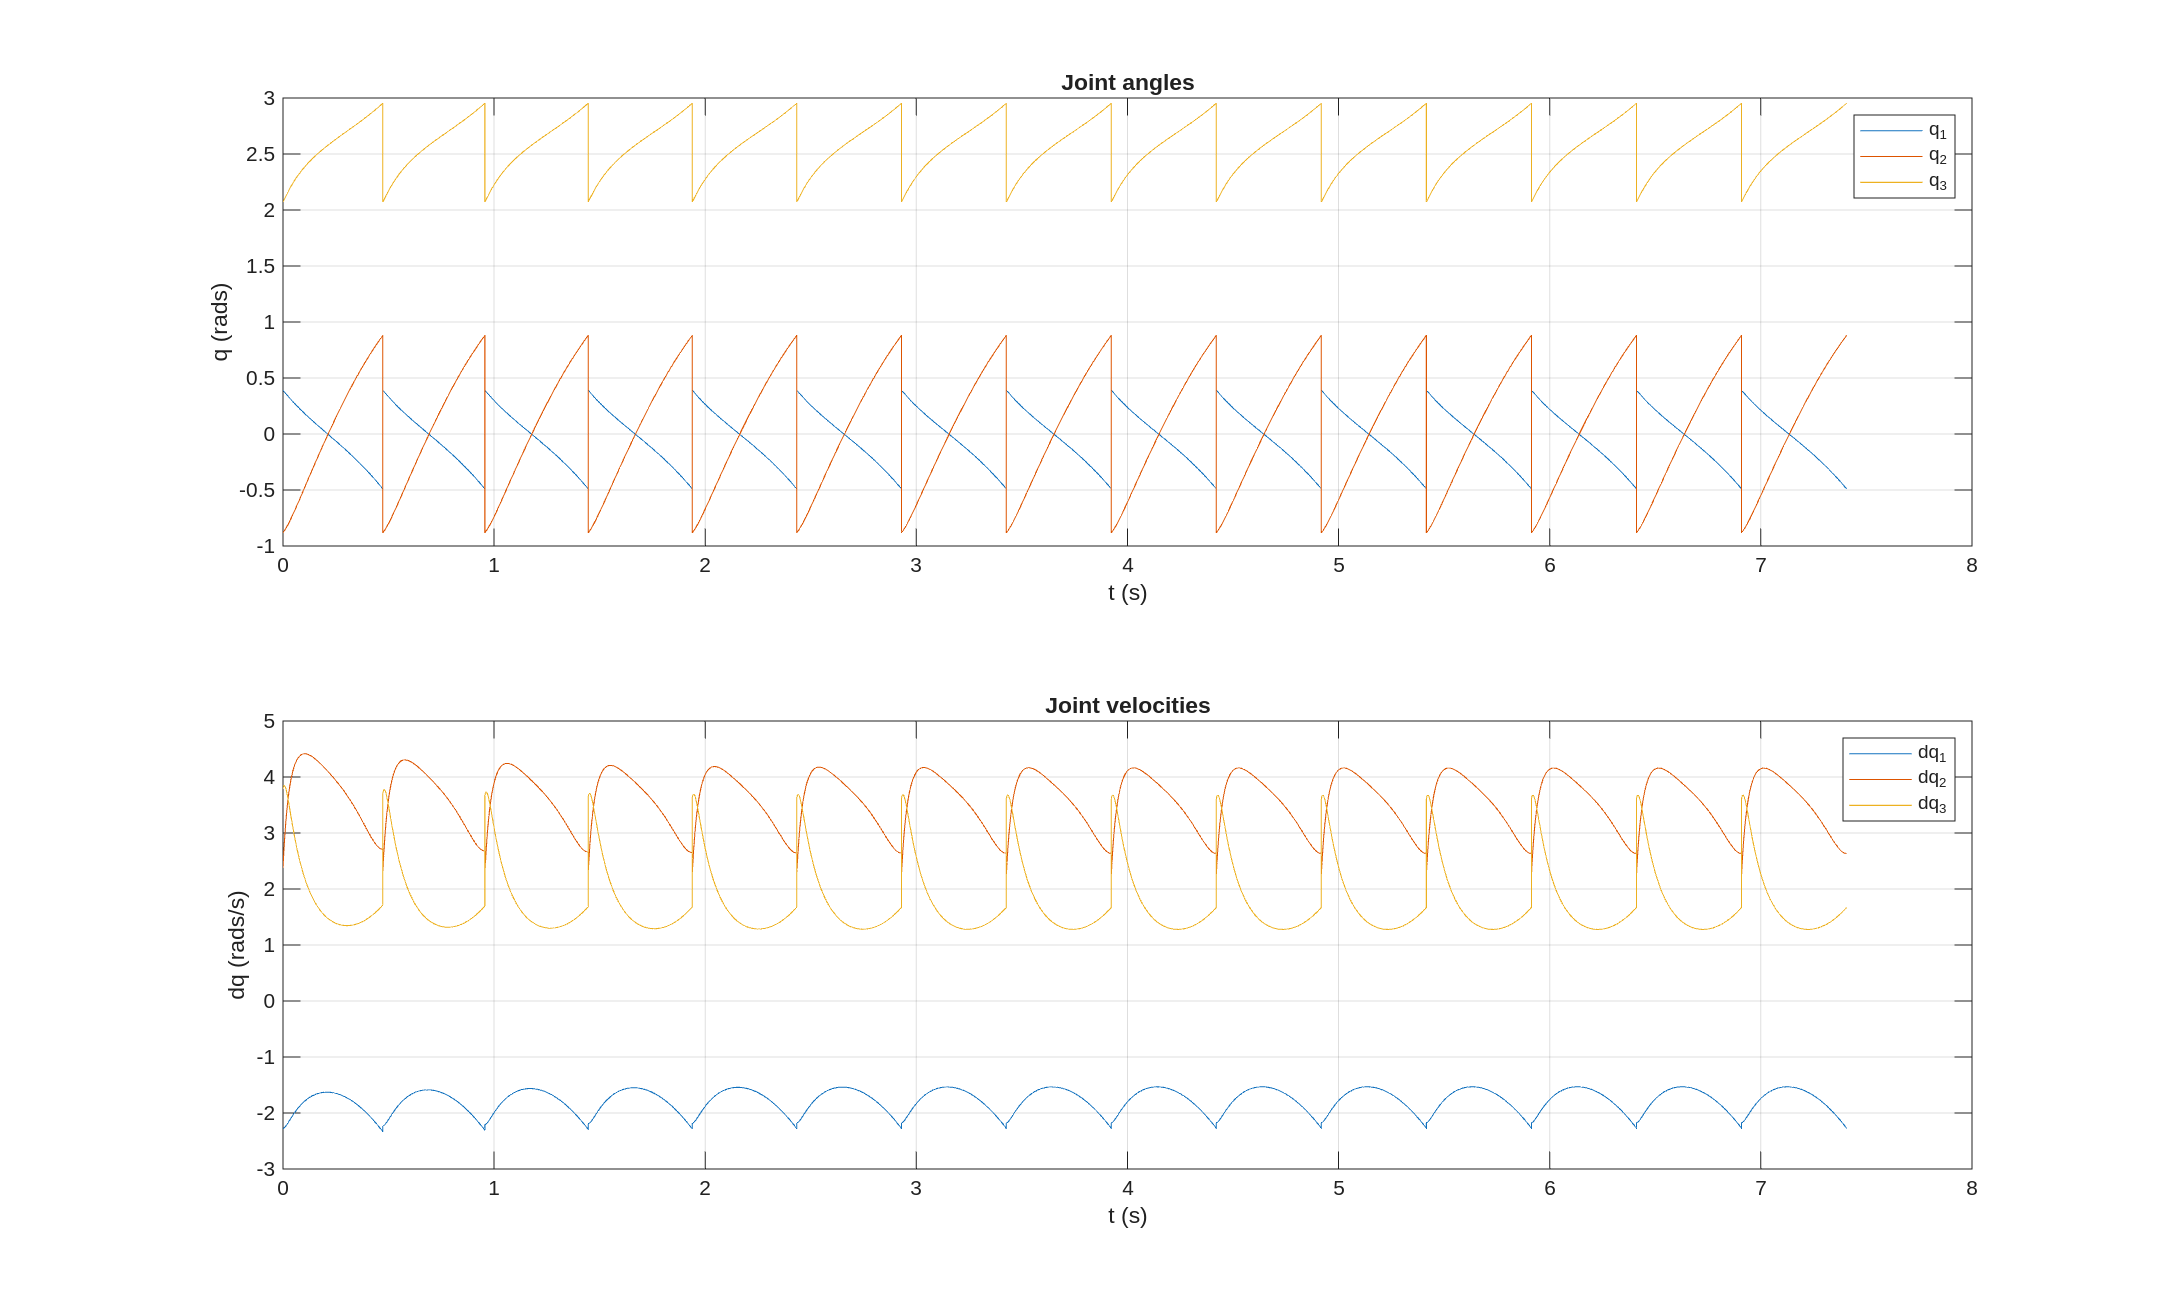
\includegraphics[width=0.9\textwidth]{q_dq.png}
    \caption{Joint angles and angular velocities.}
\end{figure}

\begin{figure}[h!]
    \centering
    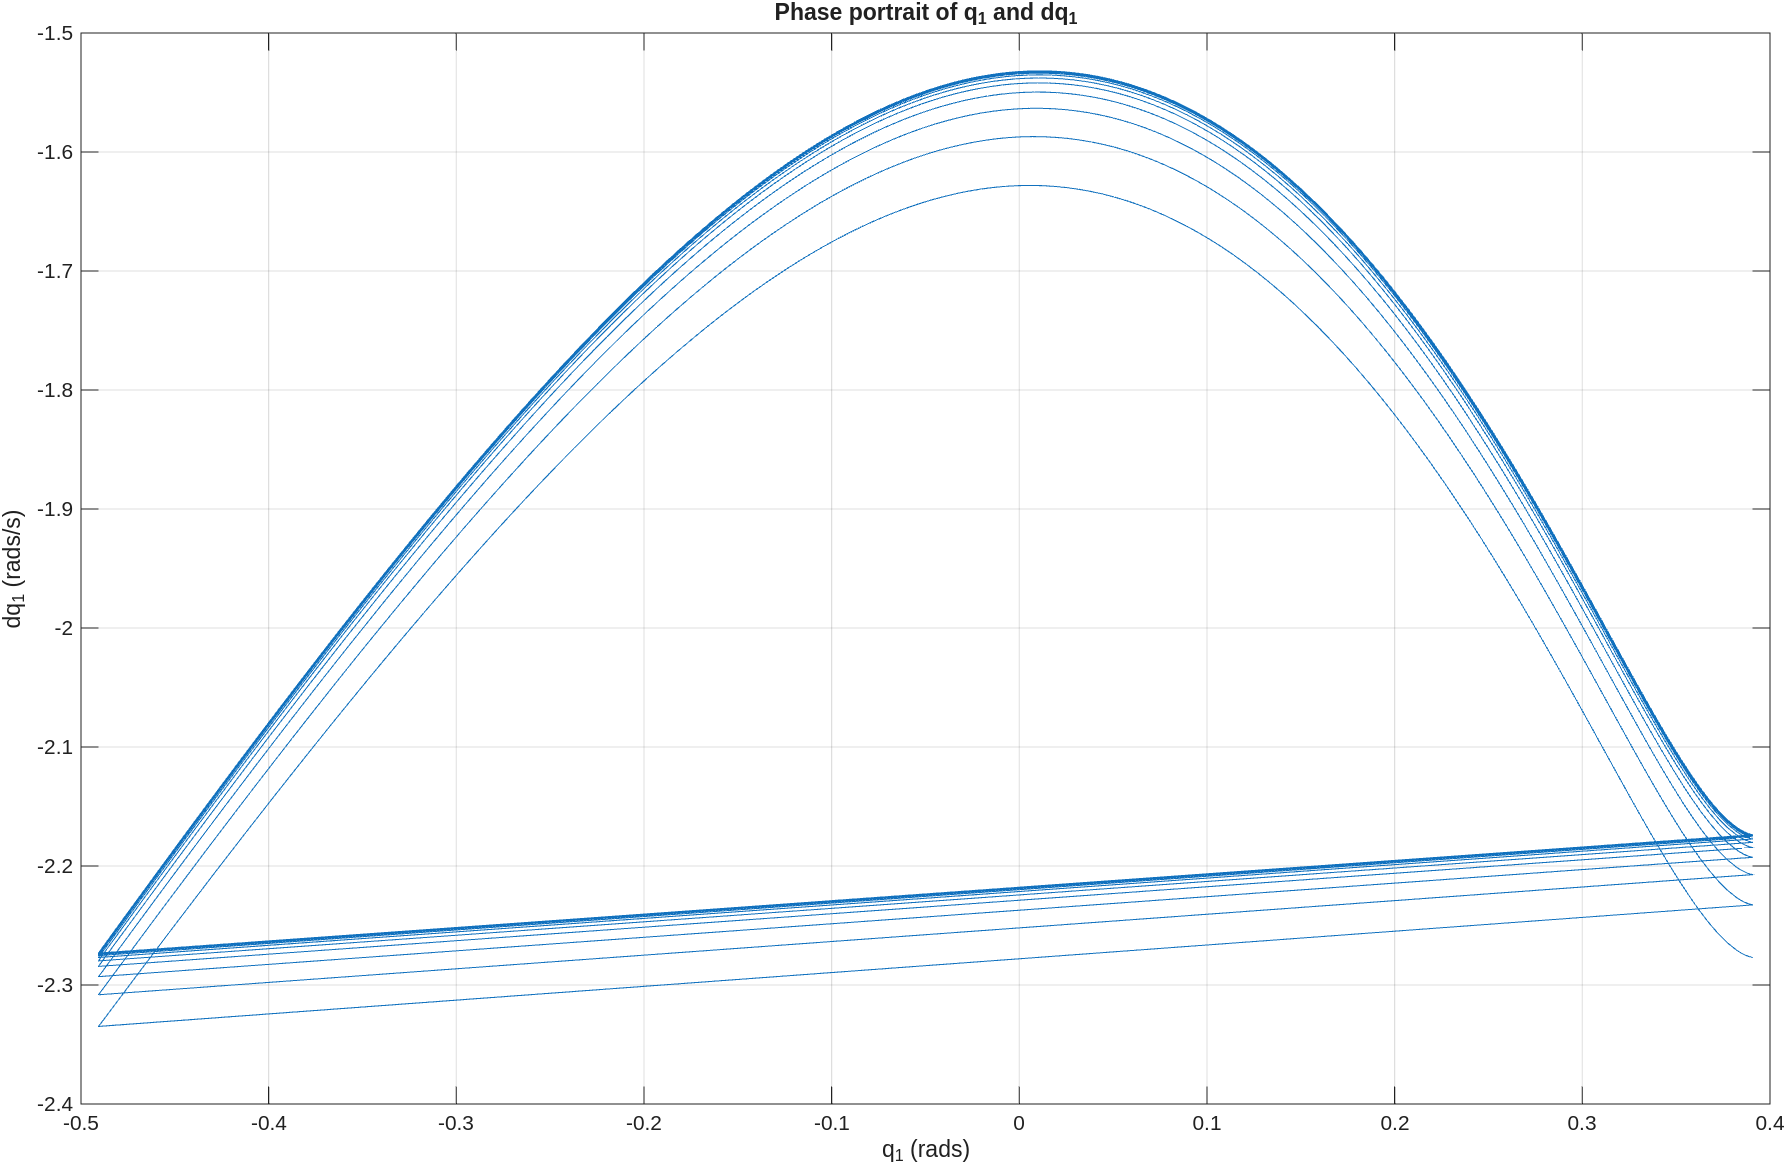
\includegraphics[width=0.9\textwidth]{FD.png}
    \caption{Phase portrait of the full dynamics ($q_1$ vs.\ $\dot{q}_1$).}
\end{figure}

\begin{figure}[h!]
    \centering
    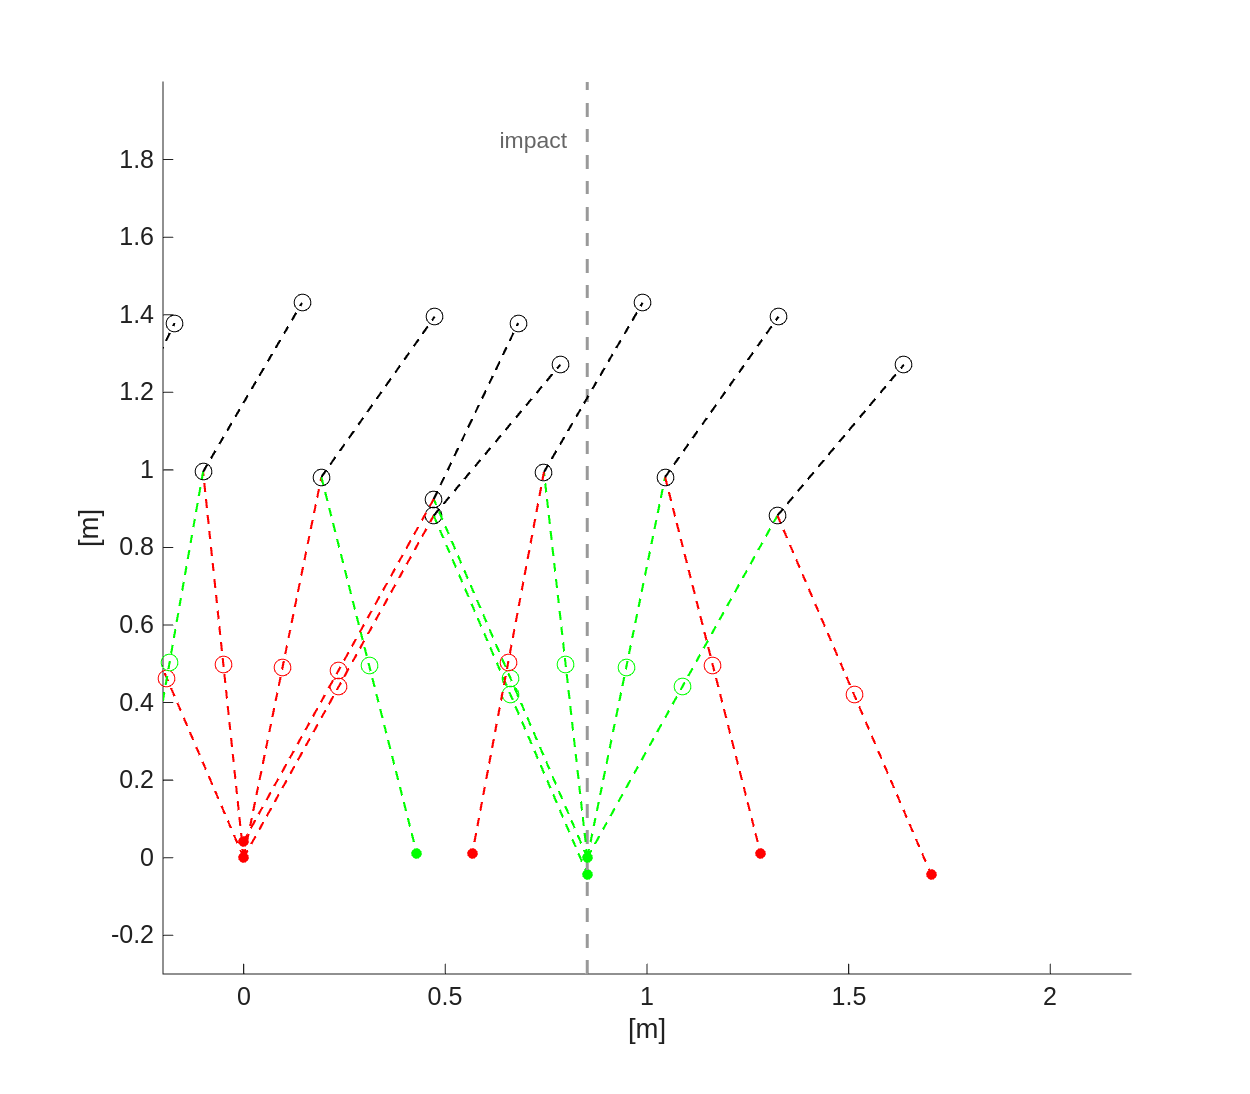
\includegraphics[width=0.9\textwidth]{anim_snapshot.png}
    \caption{Frame-by-frame animation snapshot of the walking gait.}
\end{figure}

\begin{figure}[h!]
    \centering
    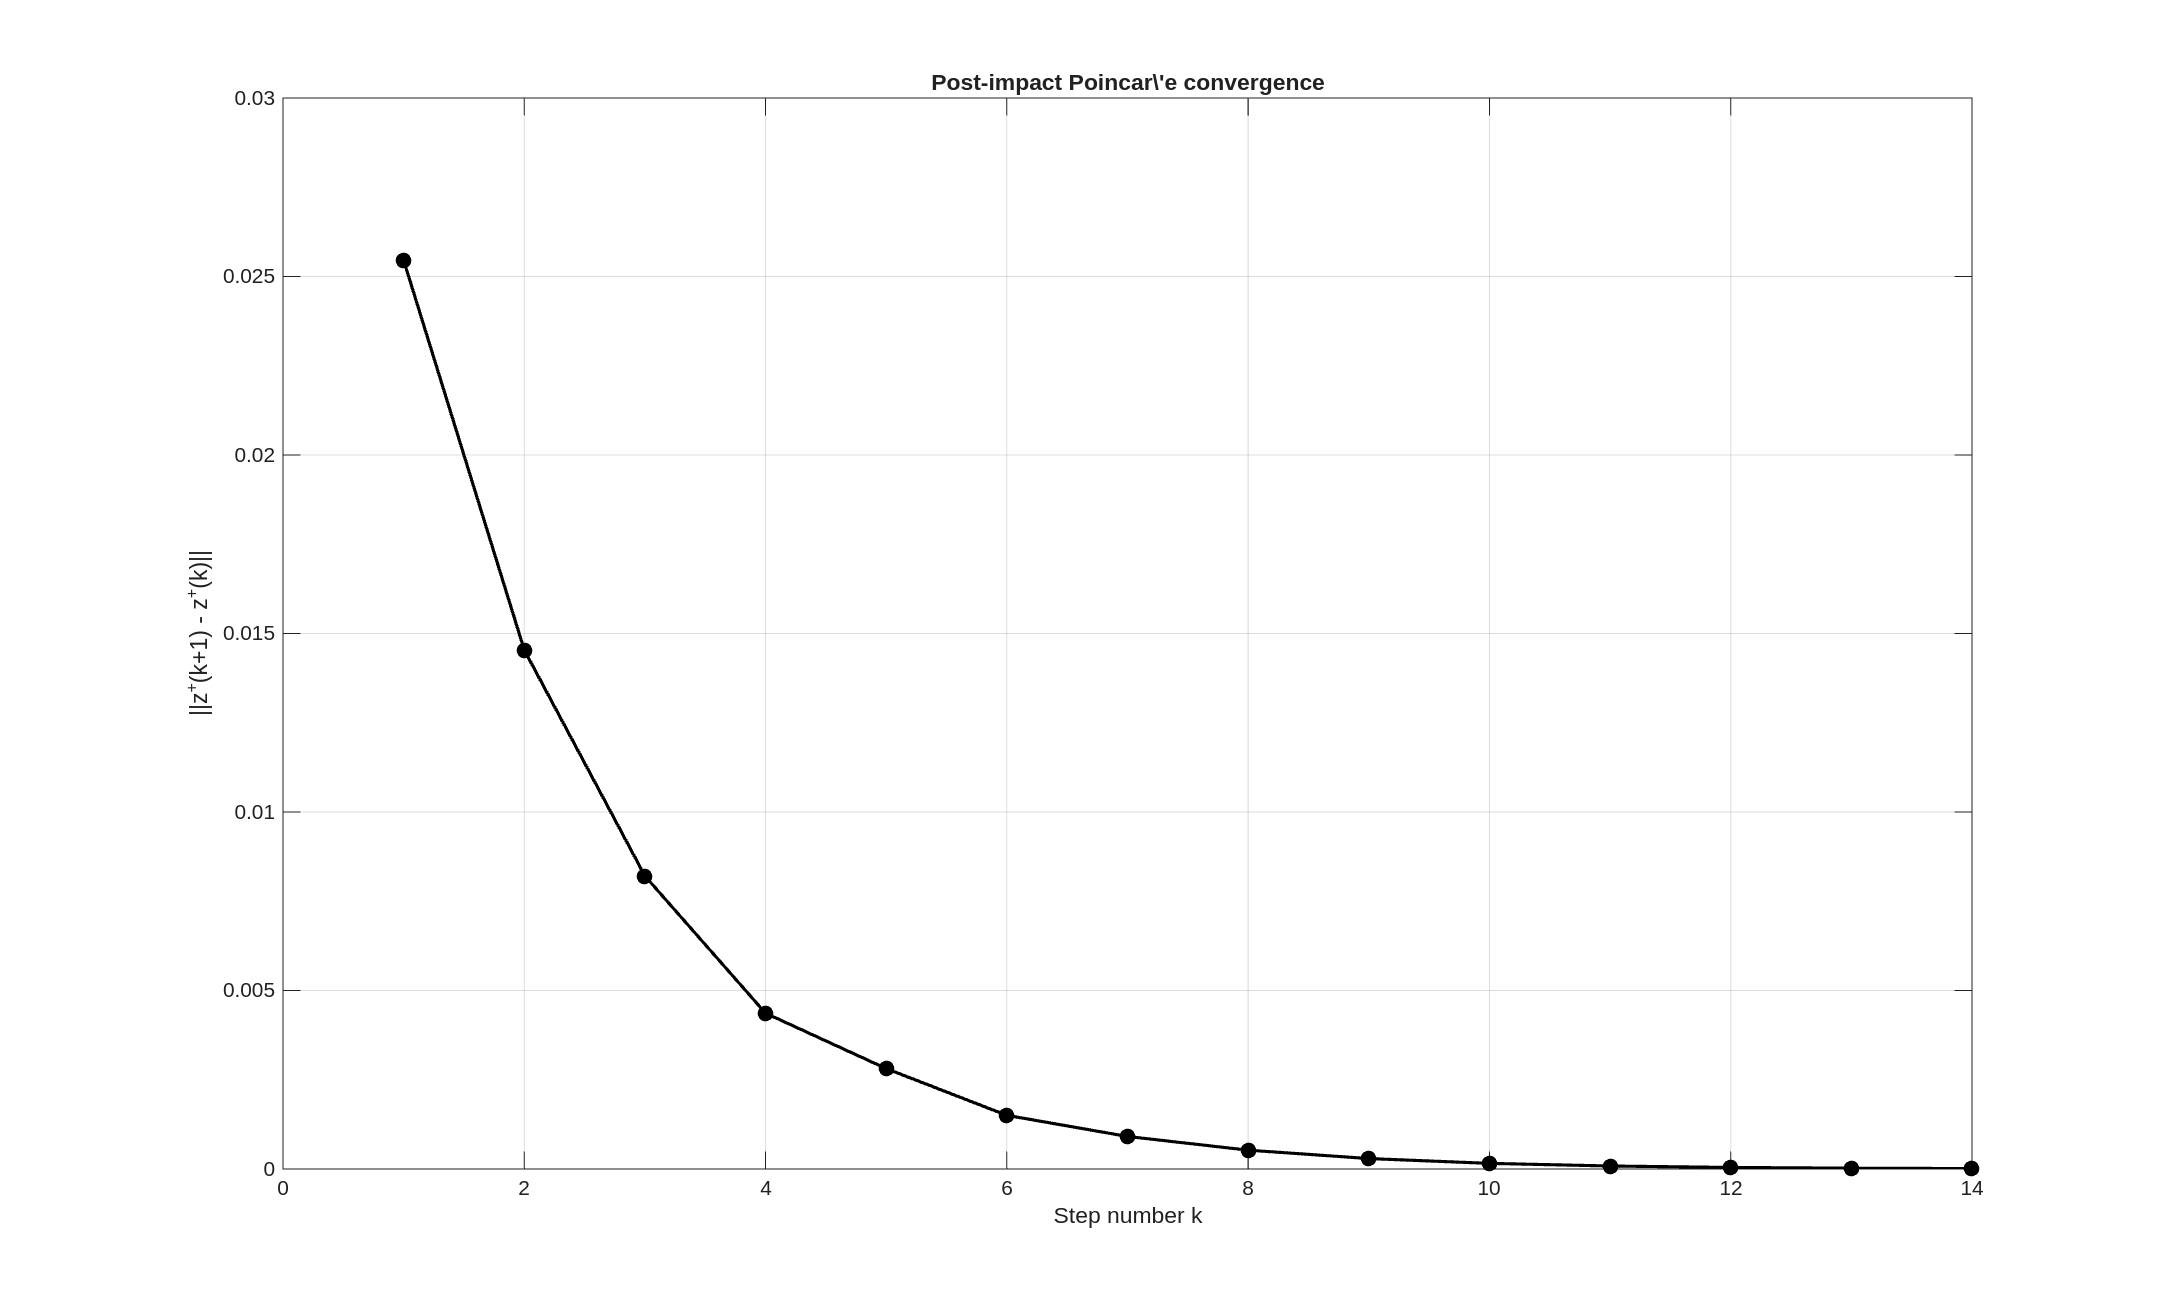
\includegraphics[width=0.9\textwidth]{pointcare_error.png}
    \caption{Step-to-step Poincar\'e map error showing convergence.}
\end{figure}

\end{document}
